\newpage
\visHeader

\begin{figure}[htbp]
    \centering
    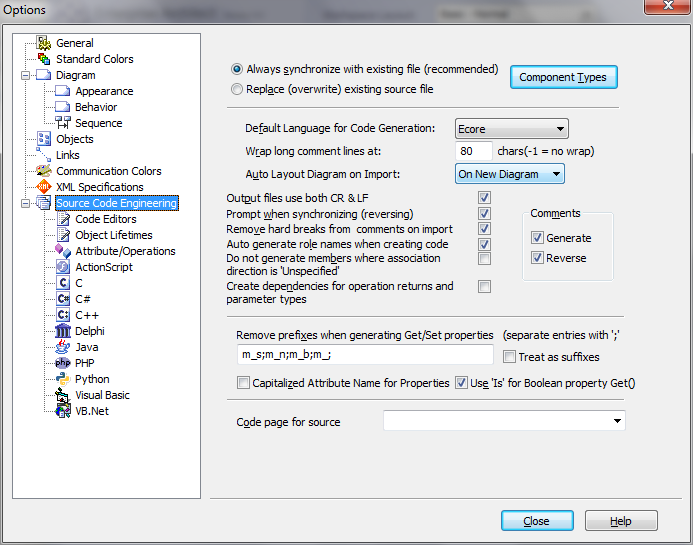
\includegraphics[width=0.8\textwidth]{standardCodeEngineering}
    \caption{Make sure you set the standard language to Ecore.}
    \label{fig_standardSCEEA}
 \end{figure}

% Repository projects are generated automatically ..
with a certain project structure according to our conventions.  
The  \texttt{model} subfolder is probably most important, and contains an  \emph{Ecore model}.  
Ecore is a metamodelling language that provides building  blocks like \emph{classes} and \emph{references} for defining the  static structure (concepts and relations between concepts) of a system.  

The  export function of our EA plugin generates a valid Ecore model from the  corresponding EA model and persists it as an XML file in the \texttt{model}  subfolder.  
In our concrete example, this is the \texttt{DoubleLinkedListLanguage.ecore} file.  
Go ahead and double-click it to open the file in a simple tree-view editor in Eclipse.  
If you are really interested in the nitty-gritty details or have a masochistic hang, right-click the file and select ``Open With/Text Editor''.

Figure~\ref{fig_fromEAtoEclipse} also depicts how the class \texttt{Node} in the EA model is mapped to the Java interface \texttt{Node}.  
Double-click \texttt{Node.java} and take a look at the methods declared in the interface.
These correspond directly to the methods declared in the modelled \texttt{Node} class.  
Indicated by the source folders \texttt{src}, \texttt{injection} and \texttt{gen}, we advocate a clean separation of hand-written (this should go in \texttt{src} and \texttt{injection}) and generated code (lands automatically in \texttt{gen}).  
As we shall see later in the handbook, hand-written code can be integrated in generated classes vio Injections. 
This is sometimes more elegant for small helper functions or necessary for String manipulation for instance.